\chapter{Gravity Model} 
%\section{Gravity Model}
\label{section:gravity-model}
As discussed in section~\ref{section:lit-review}, the Gravity model is still the standard approach to estimating OD trip distribution matrices. Its simplicity and low computational complexity makes it attractive to modelers. In modeling, it is always a good idea to develop the simplest model first. Firstly, it may be good enough, and a more complex model not required. Secondly, the errors in simpler models can aid the development of more complicated models. As such, this model will be used as a baseline to compare the destination choice models presented in section~\ref{section:destination-choice}.

\section{Design}
The gravity model is singly constrained on the origin, with the size of each zone being the sum of population and employment. The gravity model was implemented in Java, and is specified as followed:

$$ 
T_{ij} = \frac{A_j \cdot e^{-k \cdot d_{ij}}}{\sum_j^J A_j \cdot e^{-k \cdot d_{ij}}} \cdot P_i $$

Where \\
$T_{ij}$ is the number of trips between zones $i$, $j$. \\
$P_j$ is the number of trips produced in origin zone $i$.\\
$A_j$ is the attraction at destination zone $j$.\\
$k$ is the impedance factor, calibrated with the average trip distance.\\
$d_{ij}$ is the distance between zones $i$, $j$.\\

\section{Model Strata}
It is common practice to design a transport model that is in reality, a collection of separate models for heterogeneous groups of travelers, and trips. Using dis-aggregate modeling greatly assists this process, as we can cluster trips by particular attributes into more homogeneous categories. The most common attribute to categorize by is trip purpose. The TSRC provides two attributes recording trip purpose, and we use first, more general categorization for our model. This consists of 4 Categories, Business, Visit, Leisure and Other, of which only the first three are used. The category other is excluded. In figure~\ref{table:purpose-counts}, the number of trips for each category by year in the TSRC is shown. Each purpose, especially when multiple years are combined in one dataset, has a suitably large sample size to support model estimation. 

\begin{table}[H]
\centering
\caption{Sample size by trip purpose}
\label{table:purpose-counts}
\begin{tabular}{lrrrrr}
\toprule
			& 2011 	& 2012 	& 2013 	& 2014 	& Total \\
\midrule
Business 	& 1,798  & 1,640  & 1,449  & 1,341  & 6,228 \\
Leisure 	& 5,939  & 5,878  & 5,515  & 5,577  & 2,2909 \\
Visit 		& 9,057  & 8,777  & 7,962  & 7,618  & 3,3414 \\ 
\midrule
Total 		& 18,694 & 18,016 & 1,6547 & 16,071 & 6,9328 \\ 
\bottomrule
\end{tabular}%

\end{table}

\section{Calibration}
A separate model was created for each trip purpose, and calibrated to match the expected average trip distance $\bar{d}$, calculated from the trip distances recorded in the TSRC, to within 1\%. The results of the calibration are presented in table~\ref{table:gravity-calibration}. The average observed trip distance is $\bar{d}$, the average predicted trip distance $d$, and the impedance factor $k$. As measurements of error, the root mean square error (RMSE) and model correlation ($r^2$) are provided.

\begin{table}[H]
\centering
\caption{Gravity Model calibration}
\label{table:gravity-calibration}
\begin{tabular}{@{}lllll|ll@{}}
\toprule
Model & Trips & $\bar{d}$ & $d$ & $k$ & RMSE & $r^2$ \\ \midrule
   Business  & 34,229.43  &     244     &  243.20   & 0.0013 & 53.45  & 0.42  \\
   Leisure   & 83,357.94  &     149     &  148.13   & 0.0035 & 100.72  & 0.36  \\
   Visit     & 129,843.18 &     163     &  164.77   & 0.0030 & 103.65 & 0.52  \\ \bottomrule
\end{tabular}
\end{table}

\section{Results}
Figure~\ref{fig:gravity-residuals} presents an error plot, with the observed trips on the x axis, and difference between the observed and predicted on the y axis. While the three purposes cannot be compared with each other, due to the differing sample sizes, it is clear that all three models have serious errors, and are almost unusable. The predicted values should fall roughly above and below the dotted line. There is a definite pattern in the observed data, indicating that important OD pairs, ones with large numbers of trips, are strongly underestimated. The numerous OD pairs with small numbers of trips dominate the calibration to the observed average trip distance. However, this comes at the expense of model accuracy for large, important connections.

\begin{figure}[H]
\centering
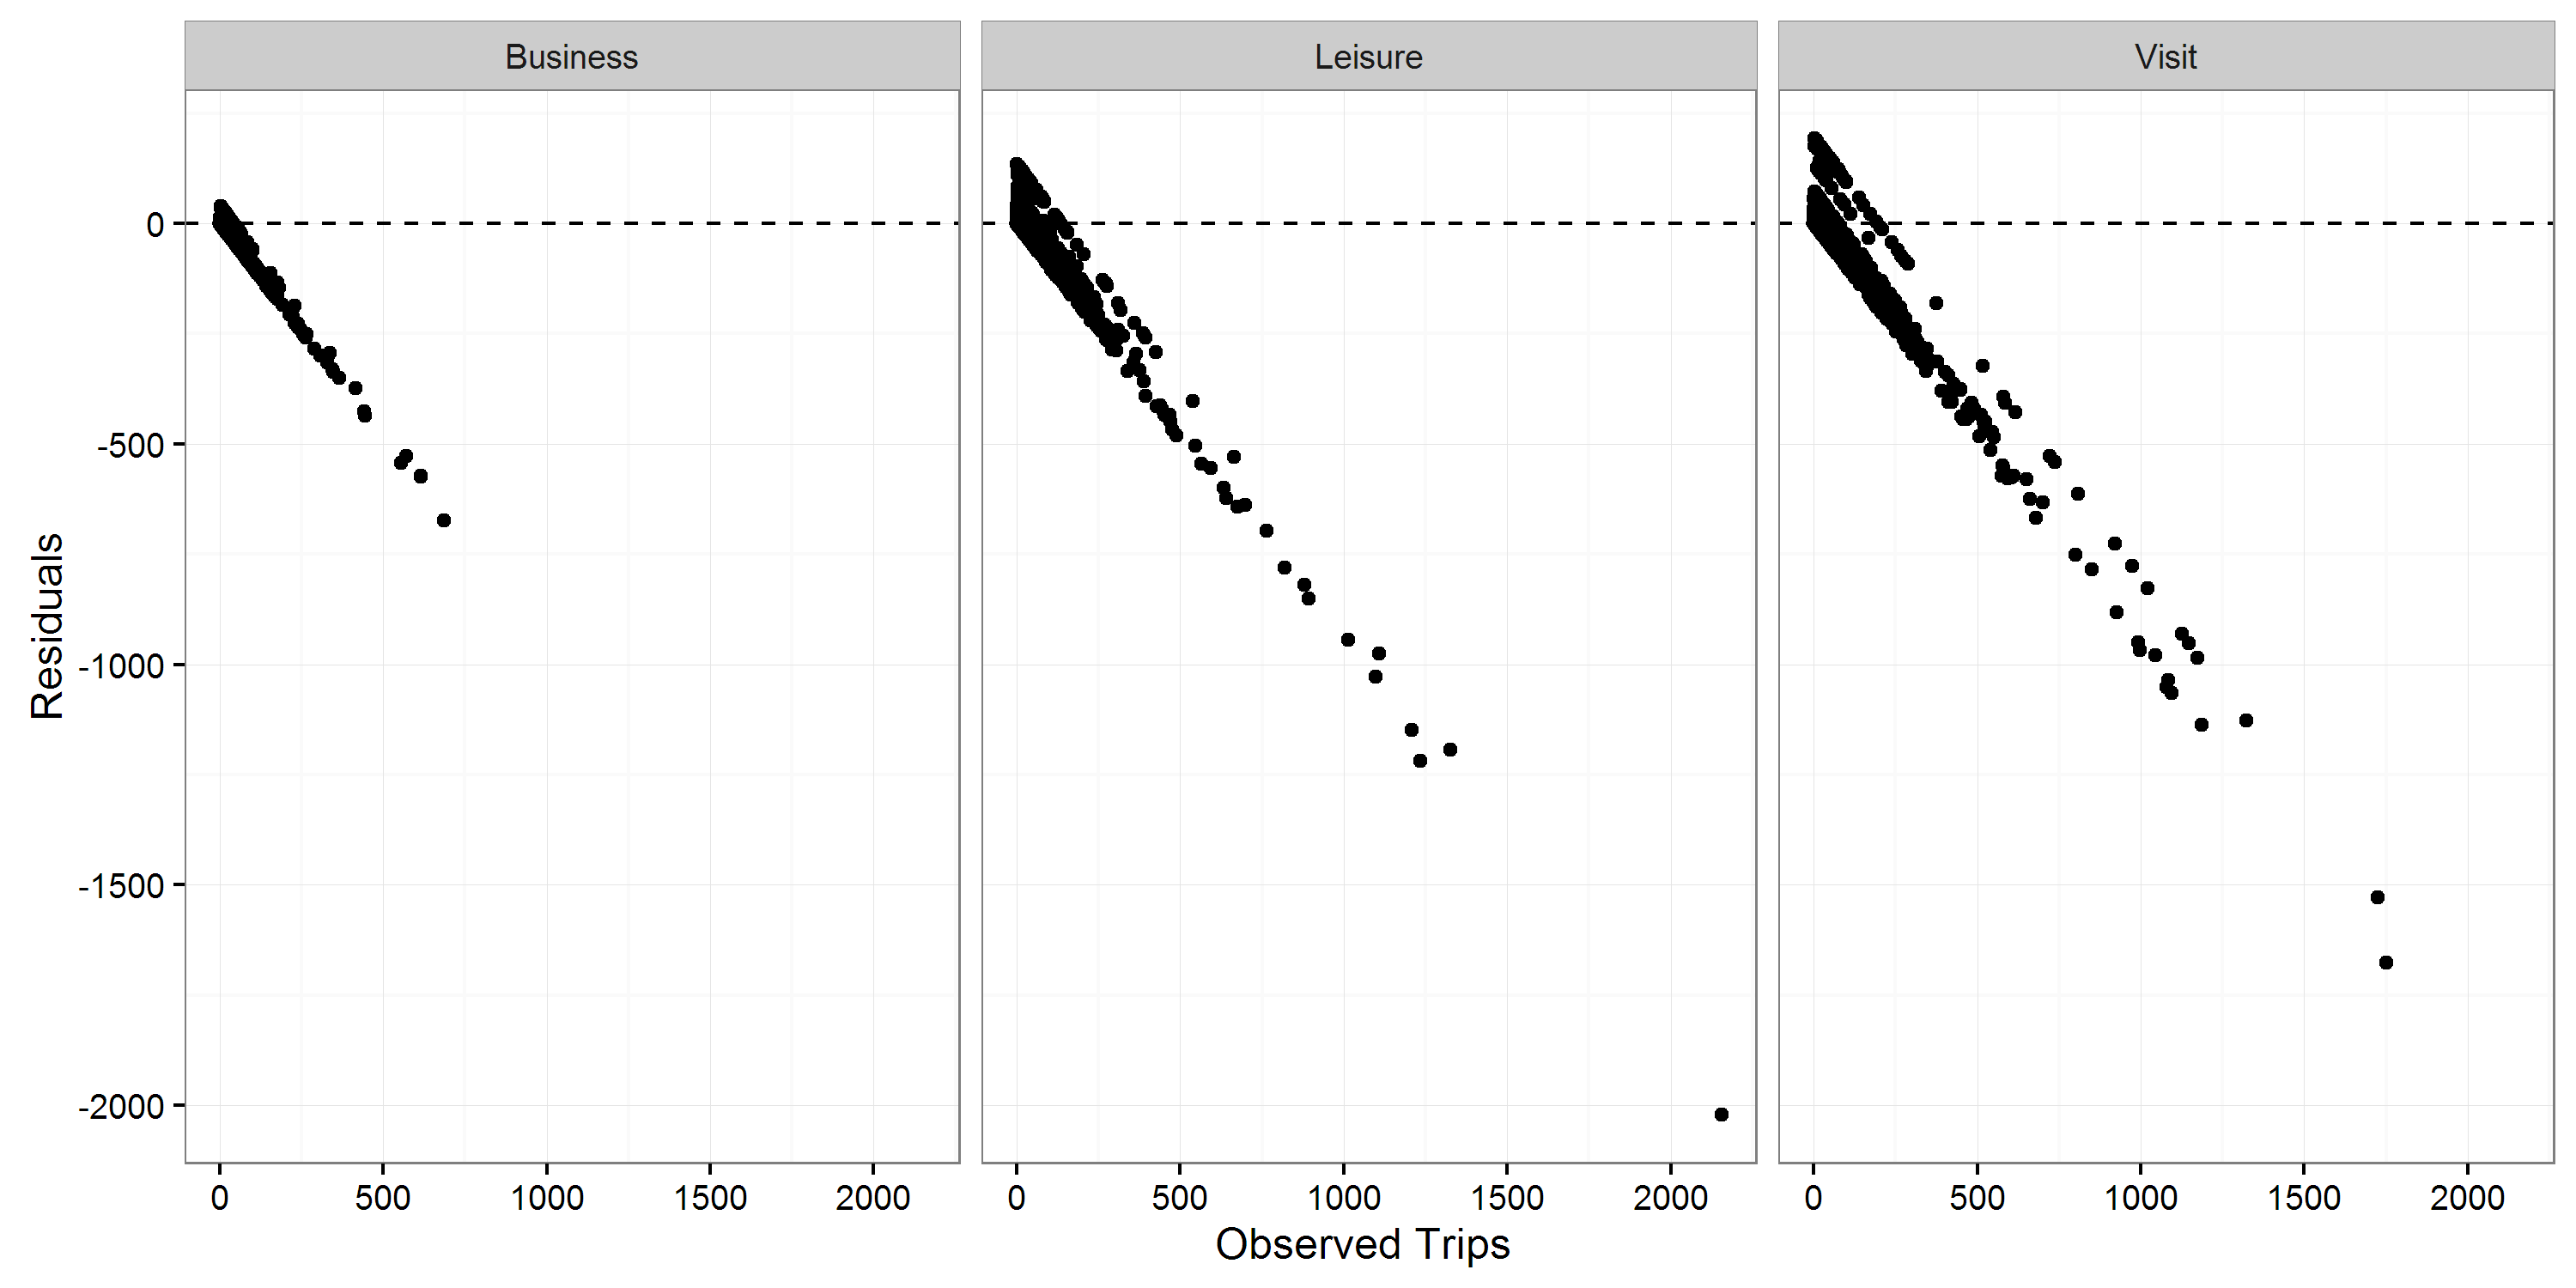
\includegraphics[width=\textwidth]{gravity_model_residuals}
\caption{Gravity model errors by observed trip count for OD pairs by trip purpose}
\label{fig:gravity-residuals}
\end{figure}

Figure~\ref{fig:gravity-errors} gives a better indication of how the model fits these important zones. On the x axis is the absolute error $|x - E(x)|$, and on the y axis, a variant of the relative error, which we call maximum relative error is plotted. 

$$\frac{|x-E(x)|}{\min(x, E(x))}$$

In the standard relative error $\frac{|x-E(x)|}{E(x)}$, only one term, $E(x)$ is present in the denominator, meaning that large underestimations produce very small relative errors, reducing the visibility of such errors in the chart. In contrast, the maximum relative error treats overestimations and underestimations equally. For this model, it is also more useful than the error plot in figure~\ref{fig:gravity-residuals}, as the error Large y values are only of concern when the x value, namely absolute error, is also large.

\begin{figure}[H]
\centering
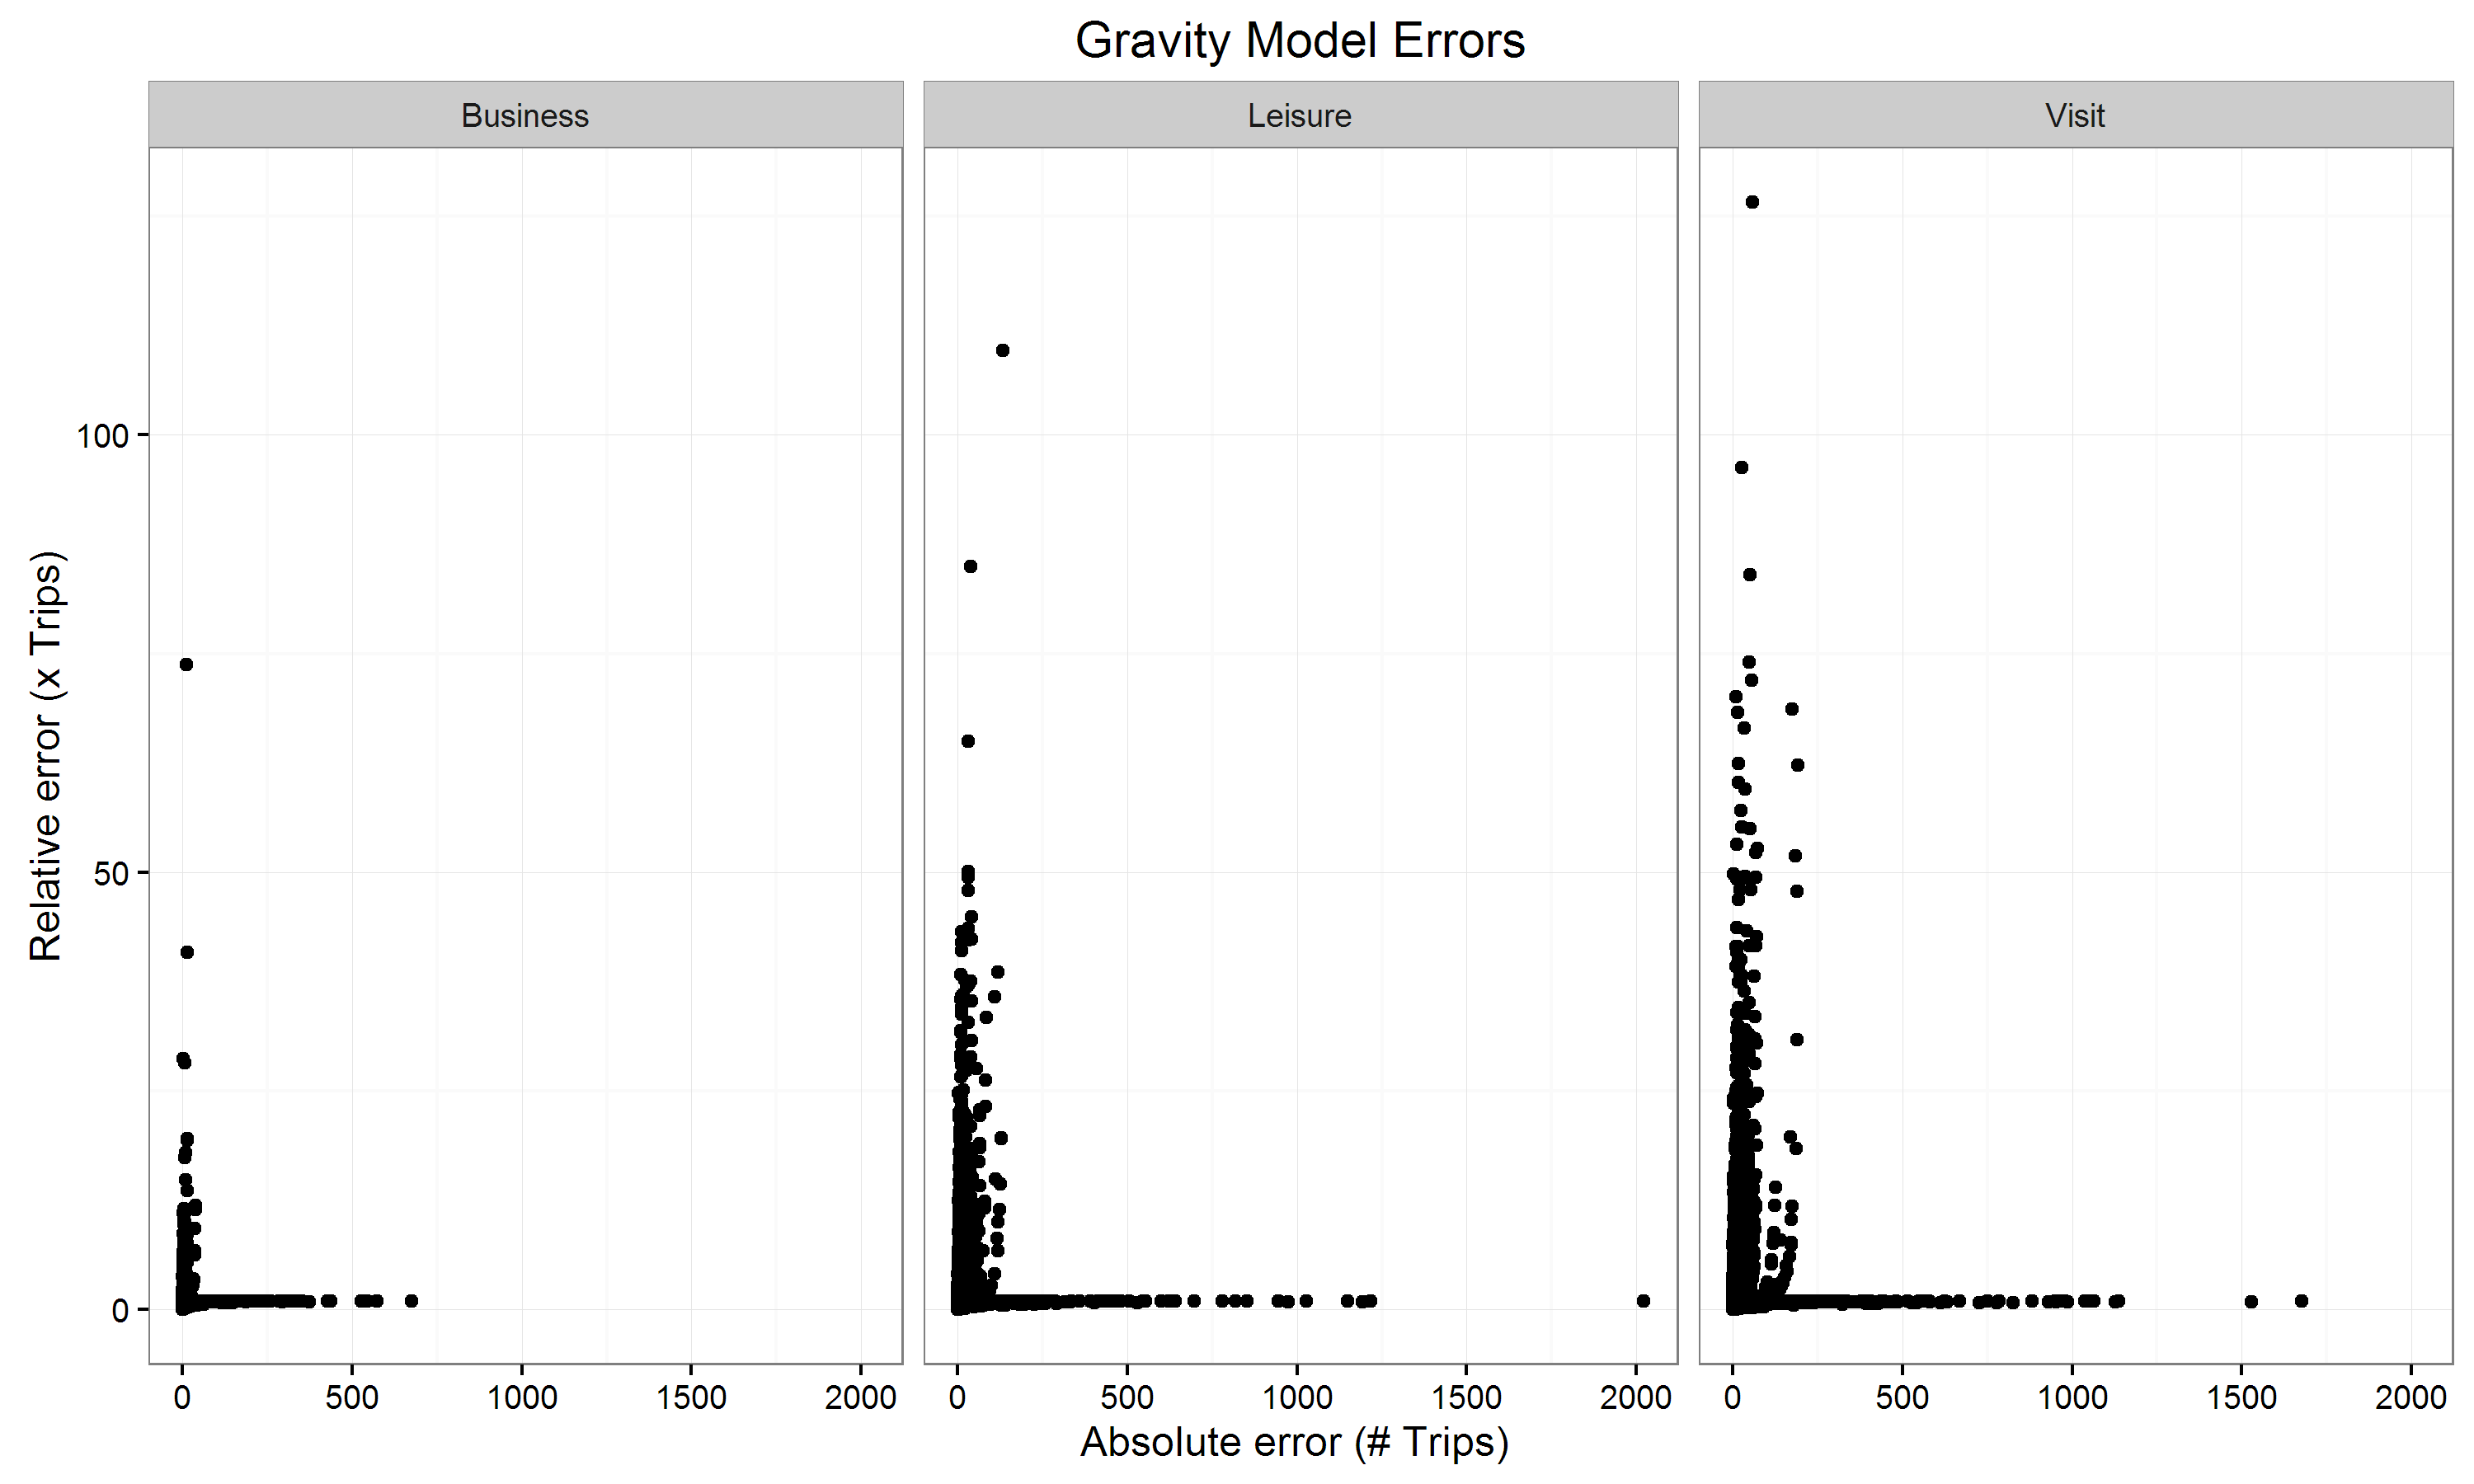
\includegraphics[width=\textwidth]{gravity_model_errors}
\caption{Maximum relative error chart for OD pairs by trip purpose}
\label{fig:gravity-errors}
\end{figure}

Large outliers are present for all three trip purposes in figure~\ref{fig:gravity-errors}. A clear weakness of the gravity model can be seen by further examining some of these outliers for the leisure purpose. The number of leisure trips originating from zones in the Toronto region to tourist destinations such as Niagara Falls and Muskoka are strongly underestimated. By its nature, the gravity model is limited in how well it can model such zone interactions, as it only takes into account one attraction factor and one impedance factor.

The propensity for leisure travelers to visit destinations with tourist attractions is clearly determined by factors other than the population and employment of the destination. The multinomial logit model of destination choice discussed in the next section adds such factors, and explores how they can be modeled.

\chapter{Destination Choice Model}
\label{section:destination-choice}
\section{Introduction}
As mentioned multiple times in this thesis already, discrete choice models are much more powerful than gravity models. However, this power comes at the cost of additional complexity, both in their set-up, estimation and application. A destination choice model gives the probability that the traveller $i$ will choose alternative $j$. 

\begin{align*}
 P_{ni} = \frac{e^{\beta x_{ni}}}{\sum_{k=1}^{K} e^{\beta x_{nk}}} 
 \intertext{where}
 x_{nk} = \left\lbrace \beta_{nk}^1,...,\beta_{nk}^K \right\rbrace and \left\lbrace w_1,...,w_K \right\rbrace \\
 K = \text{is the total number of alternatives}
\end{align*}

These $\beta$, the coefficients of the model, need to be calibrated using some optimisation function. In this thesis, this is done using Maximum Likelyhood Esimation, through the mnlogit package described in section~\ref{section:mnlogit}. The probabilities provided by an estimated model for each alternative and individual can then be used in a weighted selection of a destination for that individual. Furthermore, a trip distribution matrix can be created by summing the probabilities over the trip sample for each OD pair. This allows the model to directly be compared with aggregate models.

Firstly, the data must be transformed into the correct input structure, this process was described in section~\ref{section:mnlogit-structure}. The next step is estimation. The estimation of a discrete choice model for destination choice is much more involved than the construction of a gravity model, since modeler has almost infinite possible permutations of variables at his or her disposal. Divining the best variables is part art, part science. Some variables may be statistically significant, while adding little useful explanatory power to the model. Others may only be significant when paired with certain other variables. Rather than just present a final model, this next section elaborates on the model development process, covering the estimation, validation and implementation stages.

\section{Estimation}
In this section, the evolution of a destination choice model is presented. in \textit{m1}, a simple model based on the gravity model is presented.\textit{m2} and \textit{m3} add further interaction variables between origin and destinations. \textit{m4} explores the potential of LSBN data to improve the measure of destination utility. Finally, \textit{m5} adds the important explanatory variable of income to the model.

\subsection{Socio-economic Variables}
For the first model, the same inputs as for the gravity model are used, namely the exponential of distance $e^{-d_{ij}}$, and the combined population $p$ and employment $emp$.

The distance factor for each trip purpose was adjusted by the impedance factor $k$ estimated for the respective gravity model (see \ref{section:gravity-model}). This approach significantly improved the model, and provides a quick way to calibrate the distance coefficient without requiring the design of a more complicated GEV models.

Metropolitan areas are not homogeneous in land use patterns. There exists residential areas, and central business districts, to which people may choose to travel. However, at the spatial resolution of our zone system, these differences are hidden, resulting in a very high correlation between population and employment across the destination choice set of 98.95\%. Hence, as in the gravity model, population and employment are summed together. This value is  then log transformed, due to the long tail in the distribution (see figure~\ref{fig:pop-emp-density} in appendix (CITE). In order to simplify the further model equations, we assign a new variable for each destination
$$ civic_j = \ln\left( p_j + emp_j \right) $$

The resulting model \textit{m1}, is defined by the utility $u$ of destination $j$ for a traveler in origin $i$: 
$$ u_{ij} = \beta_1~e^{-k d_{ij}} + \beta_2~civic_j $$

where $\beta_n$ are the coefficients to be estimated by the mnlogit package. This model forms the base for further models discussed in the next sections. 

The employment data is classified by NAICS category, and models were explored where only a section of categories was included as employment. Filtering the categories of employment did not improve the model. The individual employment categories were also not considered separately as unique variables, as they were highly inter-correlated (see table~\ref{fig:pop-emp-correlation} in appendix (CITE).

The parameters of this model \textit{m1} (see table~\ref{table:m1-coeff}encouraging. All the signs are as expected, and differences in the coefficients across trip purposes are evident. A leisure trip is less likely to go towards areas of civic importance than visits or business, suggesting a preference to \enquote{escape the city}, and the trip distance is naturally less important for business travelers. For each trip purpose, the basic multinomial logit model already performs better than the gravity model, as evident in the higher correlation and lower RMSE values in table (CITE). 

%TODO: model m1 coefficients
\begin{table}[H]
\centering
\caption{\textit{m1} model coefficients}
\label{table:m1-coeff}
\begin{tabular}{@{}rlrlrlrl@{}}
  \toprule
 Parameter & \multicolumn{2}{c}{Visit} & \multicolumn{2}{c}{Leisure} & \multicolumn{2}{c}{Business} &  \\ \midrule
  $e^{-k\ d_{ij}}$ 	& 4.29 & *** & 3.86 & *** & 4.21 & *** \\ 
  $civic_j$ 		& 0.51 & *** & 0.35 & *** & 0.76 & *** \\   
   \bottomrule
\end{tabular}
\end{table}

%TODO: model m1 results

\subsection{Origin-Destination Interactions}
In this section, the model is extended with two additional variables that were introduced in section (CITE). Model \textit{m2} is specified by the utility function
\begin{align*}
u_{ij} = \beta_1~e^{-k\ d_{ij}} + \beta_2~civic_j + \beta_3~language_{ij}+ \beta_4~mm_{ij} + \beta_5~rm_{ij}
\intertext{where}
language_{ij} = language(i) \neq language(j)\\
mm_{ij} = metro(i)~\wedge~metro(j)\\
rm_{ij} = !metro(i)~\wedge~metro(j)
\end{align*}

There are 4 possible combinations of a metropolitan flag for origin and destination pairs, however, only two were selected for inclusion in the model. The flag that identifies trips leaving metropolitan areas,$mr_{ij}$, results in an unsolvable model, all other combinations, other than the one selected, $\beta_4~mm_{ij} + \beta_5~rm_{ij}$, also result in unsolvable models. 

The use of these two parameters add small improvements to the model, as can be seen in the lower AIC. The RMSE is almost the same between the models. Table~\ref{table:m2-coeff} presents the estimated parameters for this model. The new parameters vary strongly between trip purposes. 
$mm_{ij}$  works well for each trip purpose, with visit and leisure trips more likely to leave metropolitan areas, and business travel more likely to be inter metropolitan. However, language and $rm_{ij}$  do not work as well. They are not statistically significant for visit trips, and the coefficient value is at least an order of magnitude smaller than for the other trip purposes. Business dealings normally require a common language, and hence it is not surprising to see a negative coefficient for language in this category, however the language coefficient for leisure is hard to justify. Finally, $rm_{ij}$  is not significant for two trip purposes, despite working well for leisure trips. 

%%%Just include the bad model, no brackets.
% model m2 coefficients
\begin{table}[H]
\centering
\caption{\textit{m2} model coefficients}
\label{table:m2-coeff}
\begin{tabular}{@{}rlrlrlrl@{}}
  \toprule
 Parameter & \multicolumn{2}{c}{Visit} & \multicolumn{2}{c}{Leisure} & \multicolumn{2}{c}{Business} &  \\ \midrule
  $e^{-k\ d_{ij}}$ 	& 4.35 & *** & 4.57 & *** & 3.81 & *** \\  
  $civic_j$ 		& 0.52 	& *** & 0.48 & *** & 0.73 & *** \\  
  $language_{ij}$ 	& 0.05 & * & 0.58 & *** & -0.44 & *** \\ 
  $mm_{ij}$  		& -0.10 & *** & -0.99 & *** & 0.55 & *** \\ 
  $rm_{ij}$			& 0.06 & * & -0.39 & *** & -0.09 & . \\  
   \bottomrule
\end{tabular}
\end{table}
% model m2 error chart

Comparing figures~\ref{fig:gravity-errors} and (Ref m2), we can see the how many outliers have been significantly brought back towards the origin, indicating an improvement in the model. However, there are still some significant outliers, with a sample of the largest in table~\ref{table:m2-error-table} in appendix (CITE). These outliers fall into two categories:
\begin{itemize}
\item Overestimation of intra-zonal trips within a metropolitan zone such as Toronto.
\item Underestimation of leisure and visit trips from metropolitan centers to tourist attractions such as Niagara Falls.
\end{itemize}

%Model m3
As seen in figure (CITE), The large intra-zonal trip counts occur in small metropolitan zones. Since we don't want to penalize intra-zonal travel in the larger zones, which is already well estimated by the model,  $mm_{ij}$  is replaced with two new variables,

	$$	
	intrametro_{ij} = \left.
  \begin{cases}
    mm_{ij}, & \text{if } i = j \\
    0, & \text{otherwise } 0 
  \end{cases}
  \right\}
	$$
  
	$$	
	intermetro_{ij} = \left.
  \begin{cases}
    mm_{ij}, & \text{if } i \neq j \\
    0, & \text{otherwise } 0 
  \end{cases}
  \right\}
	$$
	
The other zone interaction variables $language_{ij}$  and $rm_{ij}$  are removed in this iteration, as they weren't suitable in the previous model, and the significance of their coefficients did not improve in this iteration when combined with the two new variables $intrametro_{ij}$ and $intrametro_{ij}$. 

% latex table generated in R 3.3.1 by xtable 1.8-2 package
% Wed Nov 16 14:53:39 2016
\begin{table}[H]
\centering
\caption{\textit{m3} model coefficients}
\label{table:m3-coeff}
\begin{tabular}{@{}rlrlrlrl@{}}
  \toprule
 Parameter & \multicolumn{2}{c}{Visit} & \multicolumn{2}{c}{Leisure} & \multicolumn{2}{c}{Business} &  \\ \midrule
  $e^{-k\ d_{ij}}$ 	& 4.90 	& *** & 4.90 & *** & 4.44 & *** \\ 
  $civic_j$ & 0.56 	& *** 	& 0.52 & *** & 0.74 & *** \\ 
  $intermetro_{ij}$ & -0.08 & *** & -0.89 & *** & 0.56 & *** \\ 
  $intrametro_{ij}$ & -1.71 & *** & -2.63 & *** & -0.94 & *** \\ 
   \bottomrule
\end{tabular}
\end{table}

The parameters for the \textit{m3} model are showing in table~\ref{table:m3-coeff}. The are all significant, with the two new variables having differing magnitudes and signs, that make logical sense for the different purposes. Business shows a strong preference for travelling to other metropolitan areas, as expected. Leisure travel is also very strongly influenced by metropolitan connections, but with a negative sign. This replicates the observed explanatory power of the $rm_{ij}$ variable for leisure travel in \textit{m2}, while also working for visit and business trips as well.

In table~\ref{table:model_comparisons} we can see significant improvements throughout the model iterations across all metrics. In figure~ref{figure:m3-errors}, we can also see visually the significant improvements over the gravity model. The errors on OD pairs with small numbers of observed trips are drastically reduced, particularly for visit trips. The trend to under-estimate OD pairs with large numbers of observed trips is still evident, and this problem is tackled in the next section. 

\begin{table}[H]
\centering
\caption{Comparison of model iterations}
\label{table:model_comparisons}

% Table generated by Excel2LaTeX from sheet 'Sheet1'
\begin{tabular}{lrrrrrrr}
\toprule
\textbf{Model} & \multicolumn{1}{c}{\textit{\textbf{m0}}} & \multicolumn{1}{c}{\textit{\textbf{m1}}} & \multicolumn{1}{c}{\textit{\textbf{m2}}} & \multicolumn{1}{c}{\textit{\textbf{m3}}} & \multicolumn{1}{c}{\textit{\textbf{m4}}} & \multicolumn{1}{c}{\textit{\textbf{m5}}} & \multicolumn{1}{c}{\textit{\textbf{m6}}} \\
\midrule
\textbf{\# Coefficients} & 1     & 2     & 4     & 5     &   7    & 11 & \\
\midrule
\textbf{Loglikelyhood} &       &       &       &       &       &  &\\
Business &       & -   21,053 & -   20,930  & -   20,596  & -21,071 & -20,288 &  -20,091   \\
Leisure &       & -   86,054  & -   84,705  & -   83,663  & -81,192 & -78,038 &  -77,808   \\
Visit &       & - 117,463  & - 117,441  & - 115,666  & -116,862  & -114,557 &  -113,189  \\
\midrule
\textbf{AIC} &       &       &       &       &       & & \\
Business &       &      42,110  &      41,870  &  41,201 &  42,148  & 40,590  &   40,195   \\
Leisure &       &    172,113  &    169,420  &    167,337  & 162,396  & 156,095 &  155,638     \\
Visit &       &    234,931  &    234,893  &    231,342  & 233,731 &  229,128  &  226,393   \\
\midrule
\boldmath{}\textbf{$r^2$}\unboldmath{} &       &       &       &       &       &  &\\
Business & 0.43  & 0.62  & 0.62  & 0.73  &   0.56    & 0.77 & 0.77\\
Leisure & 0.36  & 0.47  & 0.49  & 0.56  &   0.63    & 0.80 & 0.82 \\
Visit & 0.52  & 0.69  & 0.69  & 0.80  &   0.65    &  0.82 & 0.84 \\
\midrule
\textbf{RMSE} &       &       &       &       &       &  &\\
Business & 53.45 & 45.95 & 45.75 & 39.53 &   49.76    &  37.26 & 36.98 \\
Leisure & 100.72 & 90.05 & 88.85 & 82.29 &  79.66     &  59.61 & 58.68\\
Visit & 103.65 & 87.32 & 87.34 & 69.07 &   94.23    & 65.95 & 61.35 \\
\midrule
\textbf{NRMSE (\%)} &       &       &       &       &       & & \\
Business & 0.94 & 0.81 & 0.80 & 0.70 &   0.88    & 0.66 & 0.65\\
Leisure & 1.03 & 0.92 & 0.91 & 0.84 &  0.81    & 0.61  & 0.60 \\
Visit & 0.93 & 0.78 & 0.78 & 0.62 &    0.85 &  0.59 & 0.55 \\
\bottomrule
\end{tabular}%

\end{table}

\subsection{Incorporating LBSN Data}

%TODO: shouldk this be somewhere else?
As mentioned in the previous section, the traditional socio-economic variables don't reflect \textit{why} people travel to a particular destination. People don't travel to a location purely because many people live there, but because there are more opportunities in that location. Population and employment act as proxy variables for some of these opportunities, but not all. This section incorporates data from LSBNs to improve the destination choice model.  

As seen in the model results so far, leisure trips. The TSRC data show that activities such as skiing and visiting national parks are commonly performed on long distance trips. Areas where these outdoor activities are performed often have a low population and employment, while providing other attractive features to the traveler.

The collection and processing of LSBN data from foursquare was covered in section~\ref{section:data-foursquare}. To summarize briefly, the venues were collected into the following categories for each destination:
\begin{multicols}{2}
\raggedcolumns
\begin{itemize}
\item Medical
\item Ski Area
\item Airport
\item Hotel
\item Arts
\item Nightlife
\item Outdoors
\end{itemize}
\end{multicols}

Different approaches to including the foursquare variables in the model estimation were explored, and it was found that the best approach involved taking the natural log of the check-in count for each category. Not all 

%outdoor did not work - high value for toronto and niagara, as metro centers - senic lookouts

\subsection{Income Strata}



\subsection{Final Model}


